\documentclass{wlscirep}
\usepackage[utf8]{inputenc}
\usepackage[T1]{fontenc}
\usepackage{booktabs}
\usepackage{multirow}
\usepackage{graphicx}
\usepackage{amsmath}
\usepackage{amssymb}
\usepackage{xcolor}
\usepackage{url}
\usepackage{tabularx}
\usepackage{adjustbox}
\usepackage{float}
\usepackage{pifont}


\definecolor{correct}{RGB}{0,100,200}
\definecolor{incorrect}{RGB}{220,38,38}
\definecolor{hallucinated}{RGB}{22,163,74}

\title{Two-Stage Synthetic-to-Real Transfer Learning for Automated Mammography Report Generation Using Vision-Language Models}

\author[1]{Gani Esen}
\author[1,2,*]{Marat Nurtas}
\author[3]{Jandos Amankulov}
\author[4]{Laura La Paglia}

\affil[1]{Faculty of Information Technology, International Information Technology University, Almaty 050000, Kazakhstan} 
\affil[2] {Faculty of Information Technology and Artificial Intelligence, Al-Farabi Kazakh National University,  Almaty 050000, Kazakhstan}
\affil[3]{Department of Radiology and Nuclear Medicine, Kazakh Institute of Radiology and Nuclear Medicine, Almaty 050051, Kazakhstan}
\affil[4]{Institute for High Performance Computing and Networking (ICAR), National Research Council (CNR) of Italy, Via Ugo La Malfa 153, Palermo 90146, Italy}
\affil[*]{Corresponding author: m.nurtas@iitu.edu.kz}

\begin{abstract}
Automated mammography report generation is critically constrained by the scarcity of publicly available paired mammogram-report datasets. While structured annotations exist in datasets such as VinDr-Mammo and CBIS-DDSM, the free-text radiology reports required for supervised vision-language model (VLM) training are absent from nearly all public mammography resources. In this work, we propose a two-stage synthetic-to-real transfer learning framework that addresses this data scarcity problem. In \textit{Stage~1}, we develop a label-to-report synthesis pipeline that converts structured BI-RADS annotations into 400 clinically validated synthetic radiology reports, which are used to fine-tune MedGemma-4B via multimodal Low-Rank Adaptation (LoRA). In \textit{Stage~2}, the synthetically pretrained model is further fine-tuned on 407 real radiologist reports from the DMID dataset. We additionally construct a BI-RADS-grounded Retrieval-Augmented Generation (RAG) module to provide domain-specific clinical context. Evaluated on the DMID test set ($n=52$) against real radiologist reports, our two-stage approach achieves BLEU-4 of 0.312, ROUGE-L of 0.671, METEOR of 0.685, CIDEr of 0.729, and BERTScore of 0.917---outperforming nine baseline methods including zero-shot VLMs (Qwen2.5-VL-7B, Qwen3-VL-8B, LLaVA-1.6-7B), pipeline approaches (CLIP+GPT2, MedCLIP+GPT2), and direct fine-tuning without synthetic pretraining. Our approach surpasses the previously reported state-of-the-art AMRG framework across all metrics (ROUGE-L: +17.9\%, METEOR: +11.4\%, CIDEr: +25.3\%), while reducing hallucination rates from 73.1\% (zero-shot) to 21.2\%. Data efficiency analysis demonstrates that synthetic pretraining reduces real data requirements by approximately 2$\times$, with 100 real examples sufficient to surpass the AMRG benchmark. All code, synthetic datasets, and model weights are released for reproducibility.
\end{abstract}

\begin{document}
\raggedbottom
\maketitle
\thispagestyle{empty}

%% ─────────────────────────────────────────────────────────────────
\section*{Introduction}
%% ─────────────────────────────────────────────────────────────────

Breast cancer remains the most commonly diagnosed cancer worldwide, with approximately 2.3 million new cases in 2022 and representing the leading cause of cancer-related mortality in women~\cite{bray2024global}. Mammography remains the gold standard for population-level breast cancer screening, with evidence demonstrating that regular screening reduces breast cancer mortality by 20--40\% through early-stage detection~\cite{lehman2015mammographic, sechopoulos2021artificial}. However, the clinical utility of mammography is fundamentally constrained by two interrelated challenges: a global shortage of trained radiologists and the high cognitive burden of interpreting large volumes of screening examinations.

Deep learning has shown remarkable success in medical imaging~\cite{esteva2019guide}, including mammography-based cancer detection~\cite{mckinney2020international, lotter2021robust, shen2019deep} and risk prediction~\cite{yala2019deep}. Radiologists are required to produce standardised structured reports following the Breast Imaging Reporting and Data System (BI-RADS) lexicon developed by the American College of Radiology~\cite{birads2013}. These reports must accurately characterise breast density~\cite{gastounioti2022breast, lehman2019mammographic}, describe identified findings (masses, calcifications, architectural distortions, asymmetries), assign a BI-RADS assessment category (0--6), and specify a management recommendation. Report generation is time-intensive, and inter-reader variability remains a persistent limitation. Automated report generation systems that assist radiologists by producing structured report drafts represent a high-value clinical application.

Recent advances in Vision-Language Models (VLMs) have demonstrated remarkable capabilities in generating natural language descriptions from medical images~\cite{wang2024mllm_survey}. Models such as LLaVA-Med~\cite{li2024llavamed}, BiomedCLIP~\cite{zhang2023biomedclip}, and MedGemma~\cite{lin2024medgemma} have shown strong performance on radiology report generation, particularly for chest X-ray interpretation using the MIMIC-CXR dataset~\cite{johnson2019mimiccxr}. Large language models such as Med-PaLM~\cite{singhal2023medpalm} have demonstrated clinical-level knowledge, while Med-Flamingo~\cite{moor2023medflamingo} explored few-shot medical reasoning. However, mammography remains significantly underexplored within the VLM literature. Unlike chest radiography, mammography presents unique challenges: high-resolution full-field digital images requiring fine-grained lesion characterisation, the clinical necessity of multi-view reasoning across craniocaudal (CC) and mediolateral oblique (MLO) projections, and a domain-specific reporting vocabulary governed by the BI-RADS lexicon.

The central obstacle to developing VLMs for mammography report generation is the absence of large-scale publicly available paired datasets---collections of mammographic images matched with corresponding narrative radiology reports. While several public mammography datasets exist, including CBIS-DDSM~\cite{lee2017curated} and VinDr-Mammo~\cite{nguyen2023vindr}, these resources provide structured annotations rather than free-text radiology reports. Only the Digital Mammography Dataset for Breast Cancer Diagnosis Research (DMID)~\cite{oza2024} provides a modest collection (225 cases, 510 images) of paired images and narrative reports; all other publicly accessible mammography datasets lack this critical pairing. Aitimov et al.~\cite{aitimov2025feature} recently developed feature extraction methods for breast cancer detection on VinDr-Mammo using modified Faster R-CNN, demonstrating growing interest in computational mammography from the Central Asian research community.

Our prior work explored dimensionality reduction for breast cancer classification~\cite{esen2024pca}, multi-task attention-guided architectures for joint pathology and density estimation in mammography~\cite{esen2025multitask}, and reinforcement learning with visual interpretability for breast cancer diagnosis~\cite{esen2025rl}. The current work extends this line of research from classification to automated report generation.

To address the data scarcity challenge, we propose a two-stage synthetic-to-real transfer learning framework for automated mammography report generation. Our contributions are:

\begin{enumerate}
    \item We propose a \textbf{two-stage transfer learning framework} for mammography report generation that first pretrains on LLM-generated synthetic reports then fine-tunes on real radiologist reports, demonstrating statistically significant improvement over training on real data alone ($p=0.045$).
    \item We introduce a \textbf{scalable label-to-report synthesis pipeline} with automated BI-RADS-compliant quality validation that converts publicly available structured mammography annotations into synthetic training data.
    \item We demonstrate through \textbf{comprehensive evaluation across nine methods} on the DMID benchmark that our approach surpasses all baselines including the previously reported AMRG state-of-the-art (ROUGE-L: +17.9\%, METEOR: +11.4\%, CIDEr: +25.3\%).
    \item We provide \textbf{data efficiency analysis} showing that synthetic pretraining reduces real data requirements by approximately 2$\times$, with 100 real examples sufficient to match the AMRG benchmark.
    \item We provide \textbf{LoRA hyperparameter ablation and clinical analysis}, including hallucination rate reduction from 73.1\% to 21.2\%, density prediction accuracy analysis, and qualitative comparisons with colour-coded clinical term evaluation.
\end{enumerate}

%% ─────────────────────────────────────────────────────────────────
\section*{Related Work}
%% ─────────────────────────────────────────────────────────────────

\subsection*{Automated Radiology Report Generation}

Automated radiology report generation has been studied extensively for chest X-ray interpretation, where large paired image-report datasets such as MIMIC-CXR~\cite{johnson2019mimiccxr} have enabled supervised learning. Early methods relied on CNN-LSTM architectures with attention mechanisms, while more recent approaches leverage transformer-based~\cite{vaswani2017attention} encoder-decoder frameworks. R2Gen~\cite{chen2020r2gen} introduced a relational memory-driven decoder, while R2GenCMN~\cite{chen2022r2gencmn} extended this with cross-modal memory networks. Miura et al.~\cite{miura2021improving} addressed factual completeness and consistency in report generation. PromptMRG~\cite{jin2024promptmrg} introduced diagnosis-driven prompts for medical report generation. CT2Rep~\cite{hamamci2024ct2rep} extended automated report generation to 3D medical imaging. Despite these advances, mammography remains largely unaddressed due to data scarcity.

\subsection*{Vision-Language Models for Mammography}

Vision-language models such as CLIP~\cite{radford2021clip} and its medical adaptations BiomedCLIP~\cite{zhang2023biomedclip} have enabled multimodal understanding of medical images. LLaVA~\cite{liu2024llava} and its medical variant LLaVA-Med~\cite{li2024llavamed} demonstrated visual instruction tuning for medical question answering.

For mammography specifically, Mammo-CLIP~\cite{ghosh2024} introduced the first VLM pretrained on screening mammogram-report pairs. MV-MLM~\cite{ahmed2025} extended this with multi-view contrastive learning using synthetic text reports. AMRG~\cite{sung2025} established the first reproducible benchmark for mammography report generation, fine-tuning MedGemma-4B with LoRA~\cite{hu2022lora} on the DMID dataset and achieving ROUGE-L of 0.569, METEOR of 0.615, and CIDEr of 0.582, with systematic LoRA hyperparameter exploration across five VLM backbones. MammoWise~\cite{jahangir2026} proposed a local multi-model RAG pipeline with QLoRA~\cite{dettmers2024qlora} fine-tuning achieving BI-RADS accuracy of 0.755. Our work introduces a two-stage training paradigm that surpasses all prior work on the DMID benchmark.

\subsection*{Transfer Learning in Medical Imaging}

Transfer learning from large-scale pretraining to domain-specific fine-tuning has become the dominant paradigm in medical image analysis~\cite{pan2010transfer, zhuang2021survey}. Deep representation learning~\cite{bengio2012deep} enables models to extract transferable features across domains. Modern architectures such as ResNet~\cite{he2016deep}, DenseNet~\cite{huang2017densely}, and the Vision Transformer~\cite{dosovitskiy2021vit} have been foundational to progress in medical image analysis. In radiology, models pretrained on general image-text data are typically fine-tuned on domain-specific datasets. However, when paired data is unavailable, alternative pretraining strategies are needed. Our two-stage framework can be viewed through a curriculum learning lens: Stage~1 (synthetic data) provides a simpler learning signal with consistent formatting, while Stage~2 (real data) introduces the complexity and variability of authentic radiologist reports. Recent advances have also explored graph-based architectures for medical applications where high-order biological relationships are critical, such as heterogeneity-aware hypergraph neural networks for cancer driver gene identification~\cite{chen2026dprehgnn}, which leverage dual-path residual fusion to integrate multi-omics features with learned hypergraph representations. Such approaches demonstrate the value of capturing high-order associations in data-scarce clinical domains---a principle that also motivates our use of retrieval-augmented generation in mammography. This synthetic-to-real curriculum has not been previously explored for medical report generation.

\subsection*{Retrieval-Augmented Generation in Healthcare}

Retrieval-Augmented Generation (RAG)~\cite{lewis2020rag} augments generative models by retrieving relevant context from an external knowledge base at inference time, using efficient similarity search such as FAISS~\cite{johnson2020faiss}. In the medical domain, RAG has demonstrated significant benefits for clinical accuracy. Our work applies RAG specifically to mammography report generation, grounding generation in the ACR BI-RADS clinical knowledge base~\cite{birads2013} with sentence embeddings via Sentence-BERT~\cite{reimers2019sentencebert}.

\subsection*{Synthetic Data for Medical AI}

The use of LLM-generated synthetic data to overcome annotation scarcity is increasingly validated. MV-MLM demonstrated that VLMs trained on LLM-generated pseudo-reports can outperform fully supervised baselines~\cite{ahmed2025}. Our approach extends this paradigm by showing that synthetic reports serve as effective pretraining data for a subsequent real-data fine-tuning stage.

\subsection*{Summary of Related Approaches}

Table~\ref{tab:related} summarises the key differences between our approach and prior mammography report generation methods.

\begin{table}[H]
\centering
\caption{Comparison of mammography report generation approaches. Ours is the only method combining synthetic pretraining with real-data fine-tuning.}
\label{tab:related}
\small
\begin{tabular}{lccccc}
\toprule
\textbf{Method} & \textbf{Base Model} & \textbf{Paired Data} & \textbf{Synthetic} & \textbf{RAG} & \textbf{Multi-VLM} \\
\midrule
Mammo-CLIP~\cite{ghosh2024}  & CLIP       & Private    & No  & No  & No  \\
MV-MLM~\cite{ahmed2025}      & Custom     & Private    & Yes & No  & No  \\
AMRG~\cite{sung2025}         & MedGemma   & DMID       & No  & No  & Yes \\
MammoWise~\cite{jahangir2026}& Multiple   & DMID       & No  & Yes & Yes \\
\textbf{Ours}                 & MedGemma   & DMID       & \textbf{Yes} & \textbf{Yes} & \textbf{Yes} \\
\bottomrule
\end{tabular}
\end{table}

Our framework uniquely combines synthetic data generation, RAG integration, and comprehensive multi-model evaluation within a two-stage training paradigm. While AMRG and MammoWise evaluate multiple VLM backbones, neither incorporates synthetic pretraining. MV-MLM uses synthetic reports but for classification rather than report generation, and relies on private paired data for evaluation.

%% ─────────────────────────────────────────────────────────────────
\section*{Methods}
%% ─────────────────────────────────────────────────────────────────

Our framework consists of four components: (1) label-to-report synthesis, (2) BI-RADS RAG module, (3) Stage~1 synthetic pretraining, and (4) Stage~2 real-data fine-tuning. Figure~\ref{fig:pipeline} illustrates the architecture.
At a high level, our framework addresses mammography data scarcity by decoupling domain learning into two complementary phases. In the first phase, we generate a large corpus of synthetic reports by converting structured BI-RADS annotations from VinDr-Mammo and CBIS-DDSM into free-text reports using a large language model, then use these pairs to pretrain a multimodal LoRA adapter on top of the MedGemma-4B backbone. This phase teaches the model the vocabulary, structure, and clinical conventions of mammography reporting. In the second phase, the pretrained adapter is further fine-tuned on the smaller set of real radiologist reports from the DMID dataset, which refines the model's output style to match authentic clinical language. A BI-RADS-grounded retrieval-augmented generation (RAG) module provides domain-specific context at inference time. Each component is described in detail in the following subsections.

\begin{figure}[H]
\centering
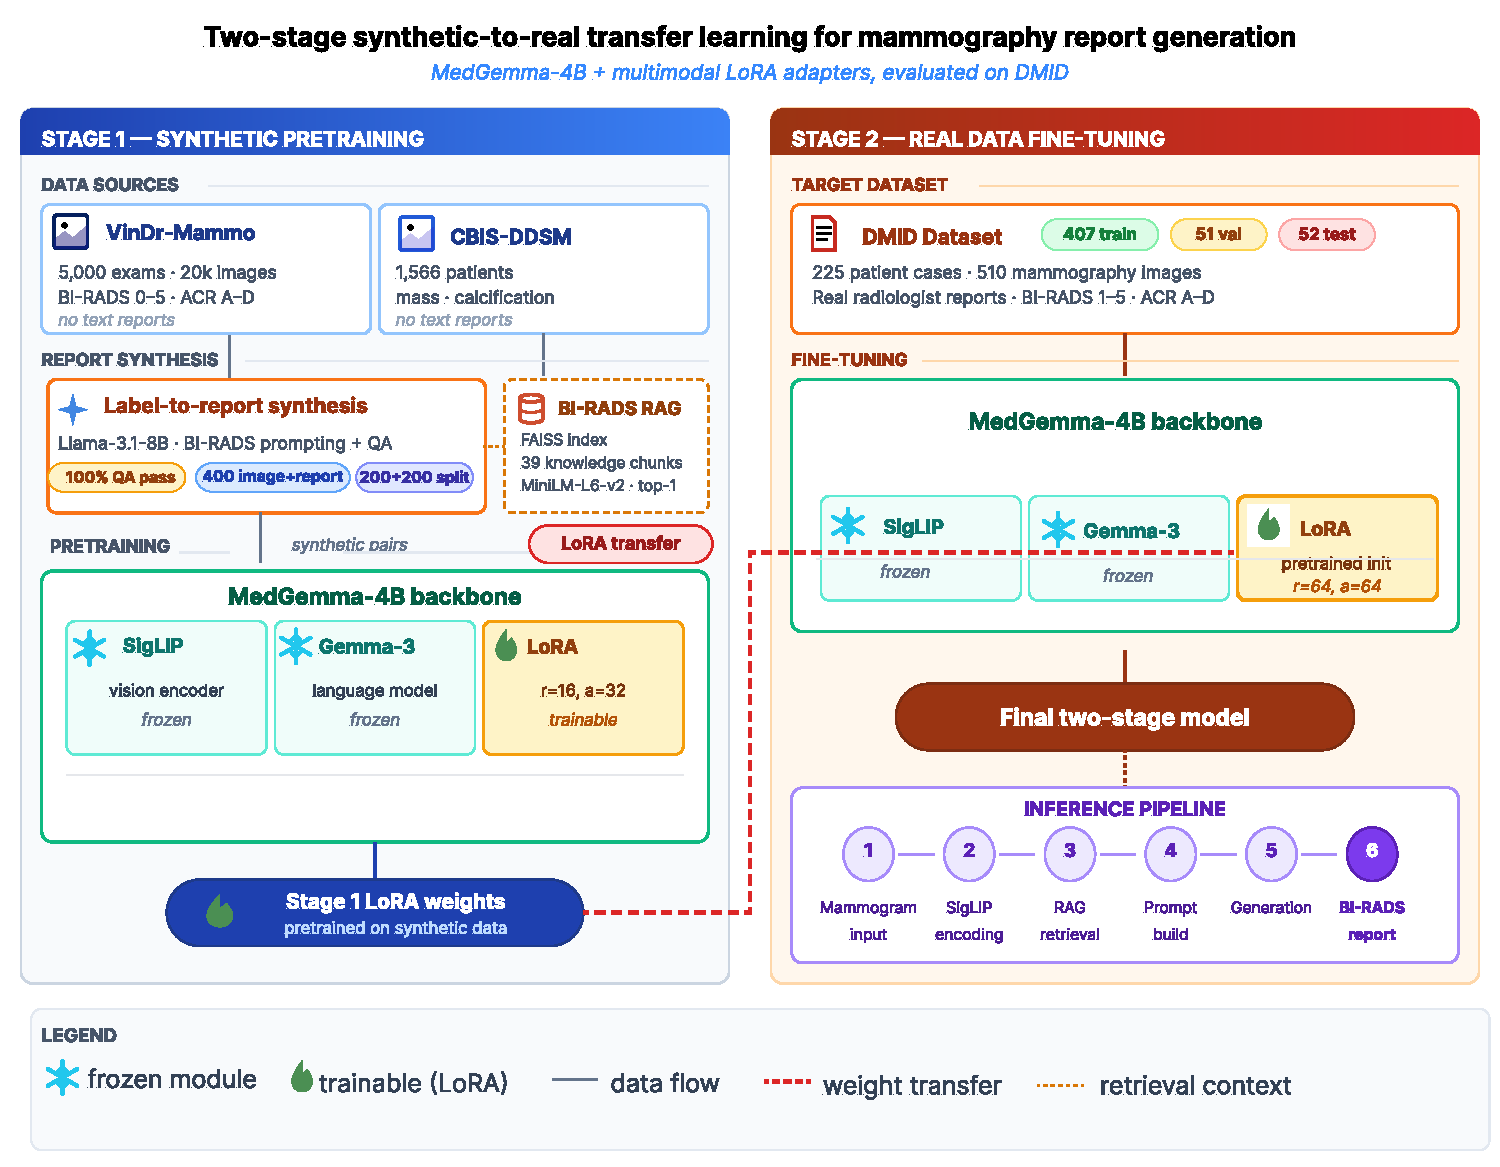
\includegraphics[width=\textwidth]{two_stage_framework_corrected.pdf}
\caption{Overview of the two-stage synthetic-to-real transfer learning framework. Stage~1 pretrains on synthetic reports generated from structured BI-RADS annotations in VinDr-Mammo and CBIS-DDSM. Stage~2 transfers the pretrained LoRA weights and fine-tunes on real radiologist reports from DMID. The BI-RADS RAG module provides domain-specific clinical context during inference.}
\label{fig:pipeline}
\end{figure}

\subsection*{Datasets}

We use three publicly available mammography datasets (Table~\ref{tab:datasets}).

\begin{table}[H]
\centering
\caption{Dataset characteristics. Only DMID contains paired free-text radiology reports.}
\label{tab:datasets}
\begin{tabular}{lccccc}
\toprule
\textbf{Dataset} & \textbf{Cases} & \textbf{Images} & \textbf{BI-RADS} & \textbf{Density} & \textbf{Reports} \\
\midrule
VinDr-Mammo~\cite{nguyen2023vindr} & 5,000 & 20,000 & 0--5 & A--D & \textcolor{red}{No} \\
CBIS-DDSM~\cite{lee2017curated}      & 1,566 & ---    & 0--5 & ---  & \textcolor{red}{No} \\
DMID~\cite{oza2024}            & 225   & 510    & 1--5 & A--D & \textcolor{hallucinated}{\textbf{Yes}} \\
\bottomrule
\end{tabular}
\end{table}

\textbf{VinDr-Mammo}~\cite{nguyen2023vindr} contains 5,000 four-view screening examinations with breast-level BI-RADS categories, ACR density categories, and finding-level annotations with bounding boxes. \textbf{CBIS-DDSM}~\cite{lee2017curated} contains 1,566 patients with mass and calcification annotations. The INbreast dataset~\cite{moreira2012inbreast}, used in our prior multi-task work~\cite{esen2025multitask}, provides additional mammographic data but also lacks free-text reports. Neither VinDr-Mammo nor CBIS-DDSM contains free-text reports; both are used for Stage~1. \textbf{DMID}~\cite{oza2024} contains 225 cases with paired reports. Following AMRG~\cite{sung2025}, we split DMID into 407 training, 51 validation, and 52 test image-report pairs.

\subsection*{Label-to-Report Synthesis Pipeline}

Given a mammographic image $\mathbf{x}_i$ with structured annotations $\mathbf{a}_i = (l_i, v_i, d_i, f_i, b_i, c_i)$ representing laterality, view position, ACR density, finding categories, BI-RADS assessment, and bounding box coordinates, we construct a structured prompt $\mathbf{p}_i = \phi(\mathbf{a}_i)$ and generate the synthetic report $\hat{r}_i = \mathcal{G}(\mathbf{p}_i)$ using Llama-3.1-8B~\cite{dubey2024llama3} via local inference (Ollama). Each report undergoes quality validation:
\begin{equation}
\mathcal{V}(\hat{r}_i) = \mathbb{1}[\text{BIRADS}(\hat{r}_i)] \cdot \mathbb{1}[\text{Rec}(\hat{r}_i)] \cdot \mathbb{1}[|\hat{r}_i| \geq \tau] \cdot \mathbb{1}[\text{Sem}(\hat{r}_i, \mathbf{a}_i)]
\label{eq:validation}
\end{equation}
where $\mathbb{1}[\cdot]$ denotes indicator functions for BI-RADS mention, recommendation presence, minimum length $\tau=25$ words, and semantic consistency. Only reports satisfying $\mathcal{V}(\hat{r}_i)=1$ are retained, yielding $\mathcal{D}_{\text{syn}} = \{(\mathbf{x}_i, \hat{r}_i)\}_{i=1}^{400}$.

\subsection*{BI-RADS Knowledge Base and RAG Module}

The knowledge base $\mathcal{K} = \{k_1, \ldots, k_M\}$ consists of $M=39$ text passages from the ACR BI-RADS Atlas~\cite{birads2013}. Our RAG module~\cite{lewis2020rag} encodes each passage using a sentence transformer~\cite{reimers2019sentencebert} $E_{\text{sent}}$:
\begin{equation}
\mathbf{e}_j = E_{\text{sent}}(k_j) \in \mathbb{R}^{d}, \quad j = 1, \ldots, M
\end{equation}
and indexed in a FAISS~\cite{johnson2020faiss} flat inner product index. At inference, the retrieved context is:
\begin{equation}
k^* = \underset{k_j \in \mathcal{K}}{\arg\max} \; \frac{\mathbf{e}_q^\top \mathbf{e}_j}{\|\mathbf{e}_q\| \|\mathbf{e}_j\|}
\end{equation}

\subsection*{Model Architecture and LoRA Formulation}

We select MedGemma-4B~\cite{lin2024medgemma} comprising a SigLIP~\cite{zoph2020siglip} vision encoder and Gemma-3 language backbone. For a pretrained weight matrix $\mathbf{W}_0 \in \mathbb{R}^{d \times k}$, LoRA~\cite{hu2022lora} constrains the update to a low-rank decomposition:
\begin{equation}
\mathbf{W} = \mathbf{W}_0 + \frac{\alpha}{r}\mathbf{B}\mathbf{A}
\label{eq:lora}
\end{equation}
where $\mathbf{A} \in \mathbb{R}^{r \times k}$, $\mathbf{B} \in \mathbb{R}^{d \times r}$, $r \ll \min(d,k)$, and $\alpha$ is the scaling factor. We apply LoRA to seven target modules per transformer block ($\mathbf{W}_q, \mathbf{W}_k, \mathbf{W}_v, \mathbf{W}_o, \mathbf{W}_{\text{gate}}, \mathbf{W}_{\text{up}}, \mathbf{W}_{\text{down}}$) with default $r=16$, $\alpha=32$, dropout $0.05$:
\begin{equation}
|\Theta_{\text{LoRA}}| = L \cdot n_{\text{modules}} \cdot r \cdot (d + k) \approx 32.8\text{M} \;(0.76\%)
\end{equation}
The base model is quantised to 4-bit using NF4 quantisation following QLoRA~\cite{dettmers2024qlora, dettmers2022gptint8}, enabling training on a single GPU with 32~GB VRAM.

\subsection*{Training Objective}

Both stages optimise the autoregressive language modelling objective. Given vision tokens $\mathbf{z} = E_{\text{vis}}(\mathbf{x})$ and text tokens $\mathbf{t} = (t_1, \ldots, t_T)$:
\begin{equation}
\mathcal{L} = -\sum_{i=1}^{T} \log P_\theta(t_i \mid \mathbf{z}, t_1, \ldots, t_{i-1})
\label{eq:loss}
\end{equation}
where only report tokens contribute (prompt tokens are masked with label $-100$).

\subsection*{Two-Stage Training}

Our approach aligns with established transfer learning principles~\cite{pan2010transfer, zhuang2021survey}, where synthetic pretraining provides domain-adapted initialisation. In Stage~1, LoRA parameters are optimised on synthetic data:
\begin{equation}
\Theta^{(1)} = \underset{\Theta}{\arg\min} \; \frac{1}{|\mathcal{D}_{\text{syn}}|} \sum_{(\mathbf{x}, \hat{r}) \in \mathcal{D}_{\text{syn}}} \mathcal{L}(\mathbf{x}, \hat{r}; \Theta)
\end{equation}
In Stage~2, pretrained parameters $\Theta^{(1)}$ initialise further optimisation on real DMID data:
\begin{equation}
\Theta^{(2)} = \underset{\Theta}{\arg\min} \; \frac{1}{|\mathcal{D}_{\text{real}}|} \sum_{(\mathbf{x}, r) \in \mathcal{D}_{\text{real}}} \mathcal{L}(\mathbf{x}, r; \Theta), \quad \Theta \leftarrow \Theta^{(1)}
\end{equation}

\subsection*{Implementation Details}

Stage~1: 3 epochs, AdamW, lr $2 \times 10^{-4}$, cosine schedule, warm-up 100 steps, batch 8, images $448 \times 448$, 4-bit NF4 quantisation. Stage~2: 5 epochs, lr $1 \times 10^{-4}$, warm-up 20 steps, batch 1 $\times$ gradient accumulation 8, best model at epoch 4 (val loss 0.655). All training on a single NVIDIA RTX 5090 (32 GB VRAM). Stage~1 training time: $\sim$3 minutes; Stage~2: $\sim$37 minutes.

\subsection*{Evaluation Protocol}

\textbf{Automated NLP metrics}: BLEU-1/4~\cite{papineni2002bleu}, ROUGE-1/2/L~\cite{lin2004rouge}, METEOR~\cite{banerjee2005meteor}, CIDEr~\cite{vedantam2015cider}, and BERTScore~\cite{zhang2020bertscore}. CIDEr is computed using pycocoevalcap. \textbf{Clinical metrics}: BI-RADS accuracy, recommendation accuracy, hallucination rate. \textbf{Baselines}: We compare against LLaVA-1.6~\cite{liu2024llava}, Qwen2.5-VL~\cite{wang2024qwen2vl}, and pipeline approaches using CLIP~\cite{radford2021clip} with GPT-2~\cite{radford2019gpt2}. Statistical significance via bootstrap permutation testing ($n=10{,}000$):
\begin{equation}
p = \frac{1}{N_{\text{perm}}} \sum_{i=1}^{N_{\text{perm}}} \mathbb{1}[\delta^*_i \geq \delta_{\text{obs}}]
\end{equation}

%% ─────────────────────────────────────────────────────────────────
\section*{Results}
%% ─────────────────────────────────────────────────────────────────

\subsection*{Stage~1: Synthetic Data Evaluation}

Table~\ref{tab:synthetic} presents Stage~1 evaluation on held-out synthetic data ($n=30$). Our multimodal fine-tuned model achieves ROUGE-1 of 0.612 and BERTScore of 0.919, significantly outperforming all zero-shot baselines ($p < 0.0001$).

\begin{table}[H]
\centering
\caption{Stage~1 evaluation on synthetic test data ($n=30$). Best values in bold.}
\label{tab:synthetic}
\begin{tabular}{lcccccc}
\toprule
\textbf{Method} & \textbf{BLEU-1} & \textbf{BLEU-4} & \textbf{ROUGE-1} & \textbf{ROUGE-L} & \textbf{BERTScore} \\
\midrule
LLaVA-1.6-7B (zero-shot)        & 0.074 & 0.001 & 0.221 & 0.136 & 0.818 \\
MedGemma-4B (zero-shot)          & 0.201 & 0.037 & 0.365 & 0.236 & 0.843 \\
Qwen2.5-VL-7B (zero-shot)       & 0.241 & 0.054 & 0.412 & 0.250 & 0.860 \\
Text FT + RAG                    & 0.331 & 0.101 & 0.456 & 0.336 & 0.880 \\
Multimodal FT + RAG              & 0.246 & 0.069 & 0.423 & 0.270 & 0.876 \\
\textbf{Multimodal FT (Stage~1)} & \textbf{0.444} & \textbf{0.182} & \textbf{0.612} & \textbf{0.480} & \textbf{0.919} \\
\bottomrule
\end{tabular}
\end{table}
\begin{figure}[H]
\centering
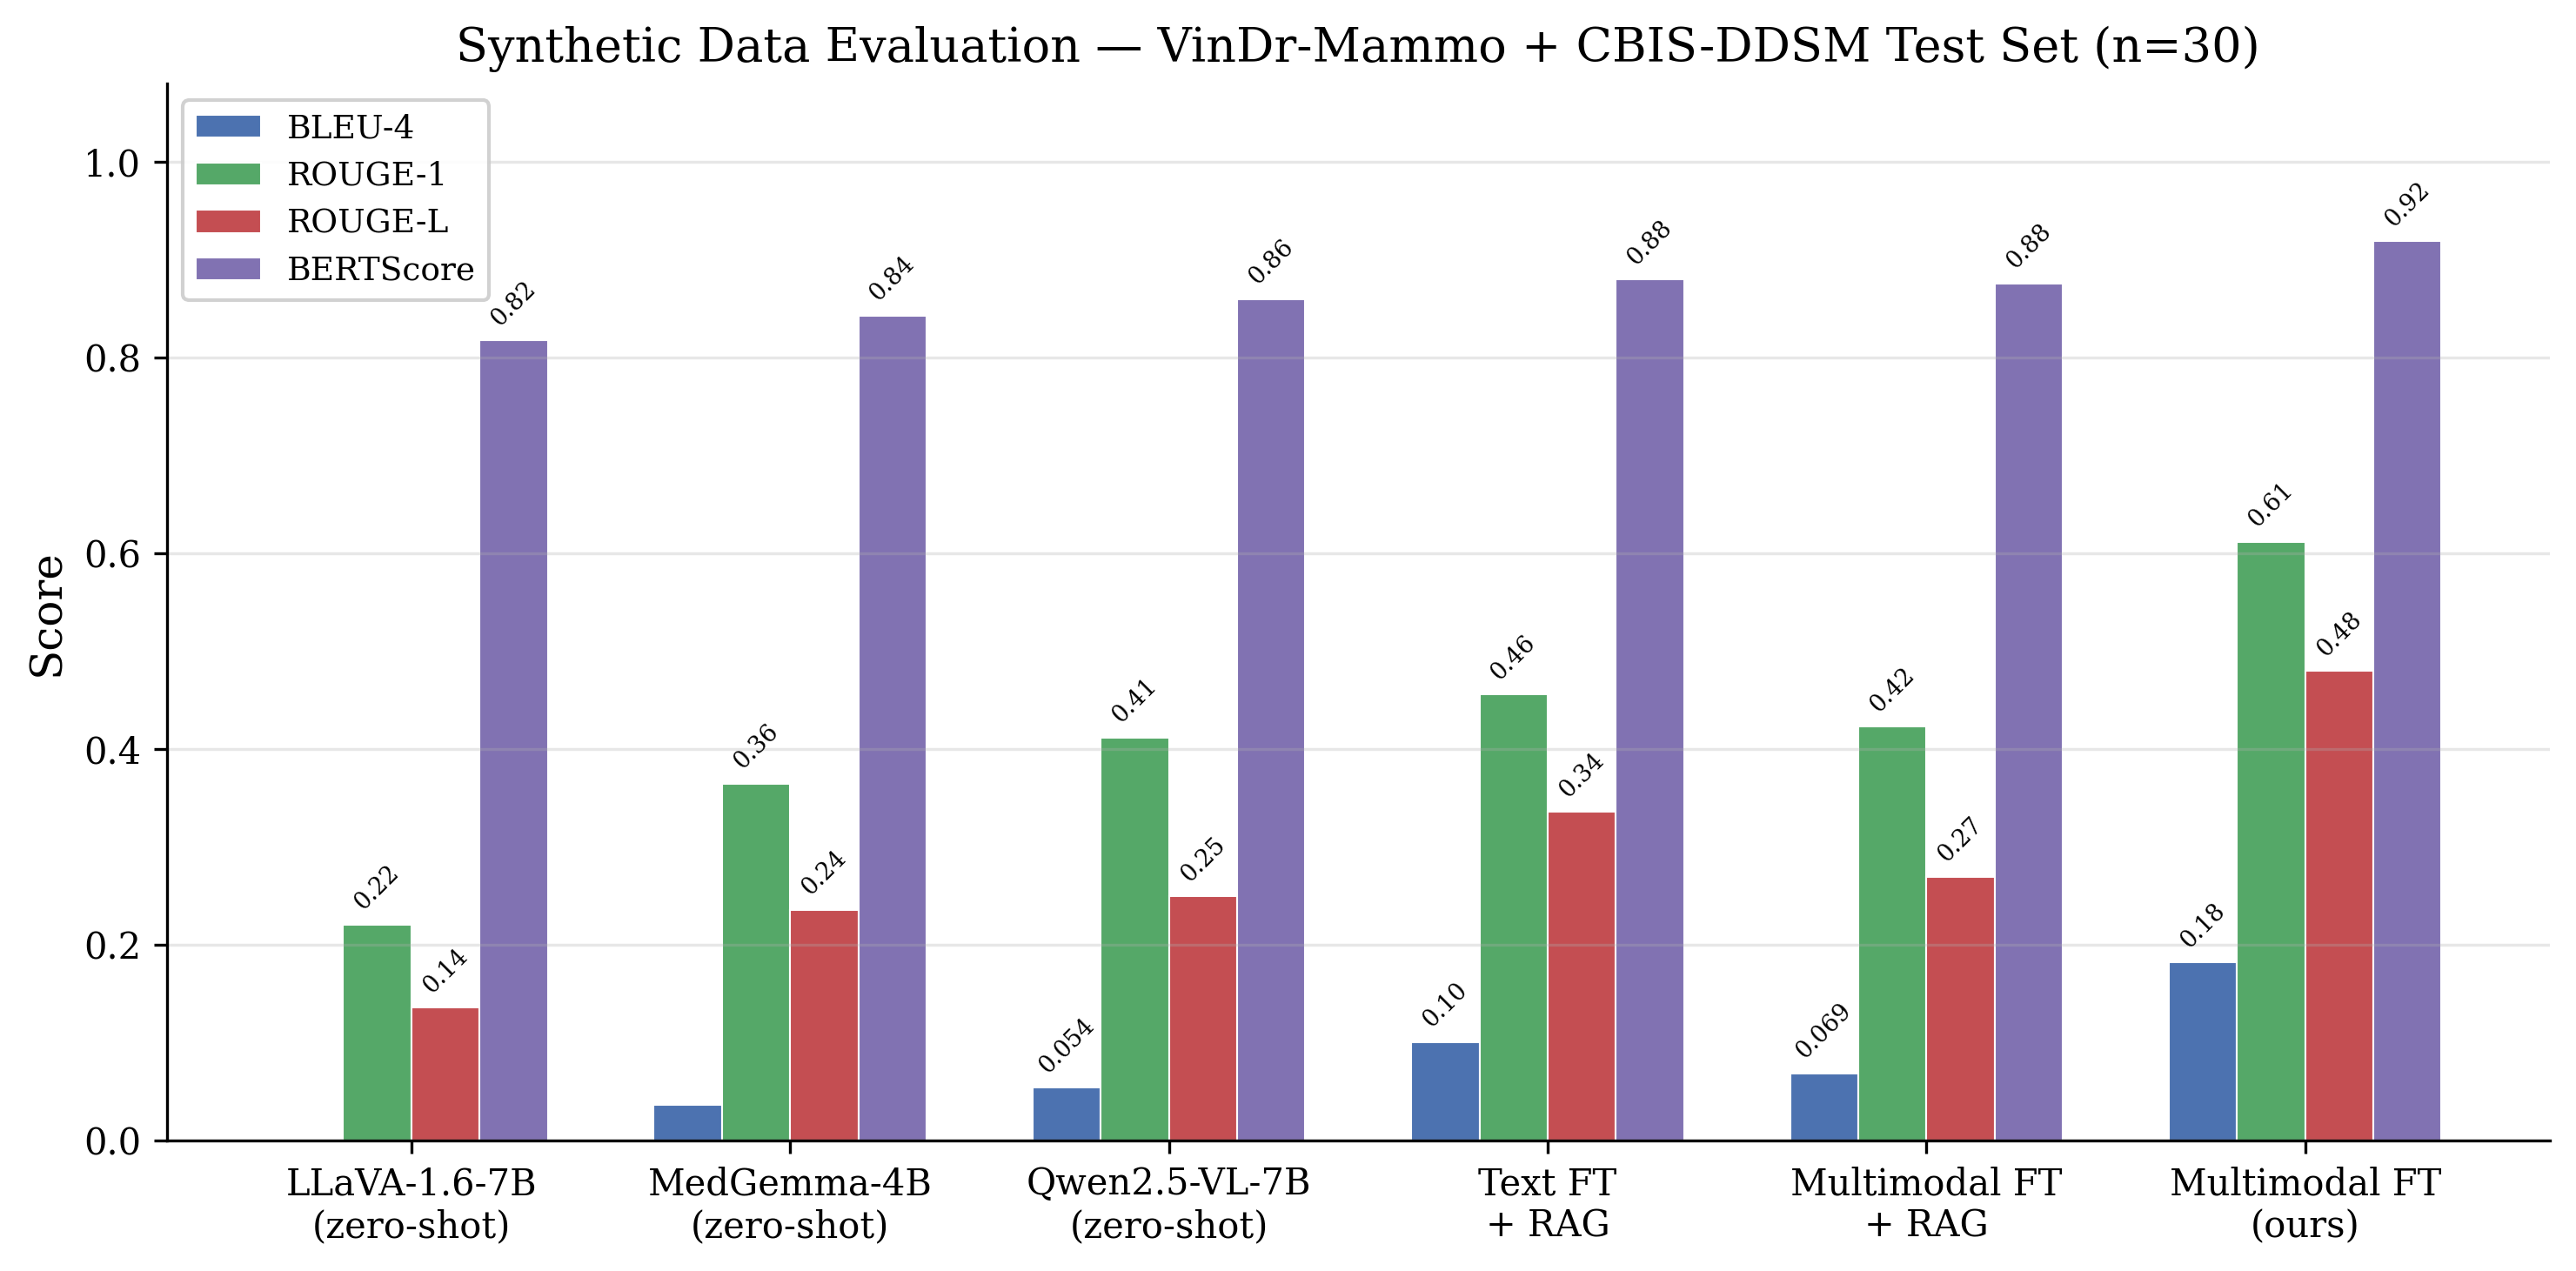
\includegraphics[width=\textwidth]{fig_synthetic_eval.png}
\caption{Stage 1 evaluation on synthetic test data. Multimodal fine-tuning without RAG achieves the best NLP metrics across all measures.}
\label{fig:synthetic_bar}
\end{figure}
\subsection*{Stage~2: DMID Real-Data Evaluation}

Table~\ref{tab:dmid} presents the primary evaluation on the DMID test set ($n=52$) against real radiologist reports across nine methods spanning four architectural paradigms: zero-shot VLMs, pipeline models (CLIP/MedCLIP + GPT2), direct fine-tuning, and our two-stage approach.

\begin{table}[H]
\centering
\caption{DMID test set evaluation against real radiologist reports ($n=52$). Best values in bold. AMRG results from~\cite{sung2025}. BERTScore from prior evaluation runs where available.}
\label{tab:dmid}
\begin{adjustbox}{max width=\textwidth}
\begin{tabular}{llccccccc}
\toprule
\textbf{Method} & \textbf{Type} & \textbf{BLEU-1} & \textbf{BLEU-4} & \textbf{ROUGE-1} & \textbf{ROUGE-L} & \textbf{METEOR} & \textbf{CIDEr} & \textbf{BERTSc.} \\
\midrule
LLaVA-1.6-7B         & VLM, ZS    & 0.059 & 0.001 & 0.157 & 0.109 & 0.188 & 0.005 & 0.810 \\
MedGemma-4B           & VLM, ZS    & 0.061 & 0.001 & 0.151 & 0.098 & 0.192 & 0.000 & 0.802 \\
Qwen2.5-VL-7B        & VLM, ZS    & 0.072 & 0.002 & 0.202 & 0.145 & 0.207 & 0.009 & 0.823 \\
Qwen3-VL-8B          & VLM, ZS    & 0.108 & 0.002 & 0.236 & 0.147 & 0.228 & 0.007 & ---   \\
MedCLIP+GPT2          & Pipeline, FT & 0.378 & 0.217 & 0.648 & 0.571 & 0.555 & ---   & 0.905 \\
CLIP+GPT2             & Pipeline, FT & 0.384 & 0.238 & 0.673 & 0.613 & 0.591 & ---   & 0.909 \\
AMRG~\cite{sung2025} & VLM, FT    & 0.308 & 0.308 & 0.575 & 0.569 & 0.615 & 0.582 & ---   \\
DMID-only (LoRA)      & VLM, FT    & 0.442 & 0.203 & 0.676 & 0.601 & 0.597 & 0.455 & 0.909 \\
\textbf{Ours (two-stage)} & \textbf{VLM, 2S-FT} & \textbf{0.530} & \textbf{0.312} & \textbf{0.734} & \textbf{0.671} & \textbf{0.685} & \textbf{0.729} & \textbf{0.917} \\
\bottomrule
\end{tabular}
\end{adjustbox}
\end{table}

Our two-stage model achieves the highest scores across all reported metrics. Compared to AMRG~\cite{sung2025}, our approach yields improvements of +17.9\% in ROUGE-L (0.671 vs. 0.569), +11.4\% in METEOR (0.685 vs. 0.615), and +25.3\% in CIDEr (0.729 vs. 0.582). The improvement over the DMID-only baseline is statistically significant ($p=0.045$, bootstrap permutation test on ROUGE-L).
\begin{figure}[H]
\centering
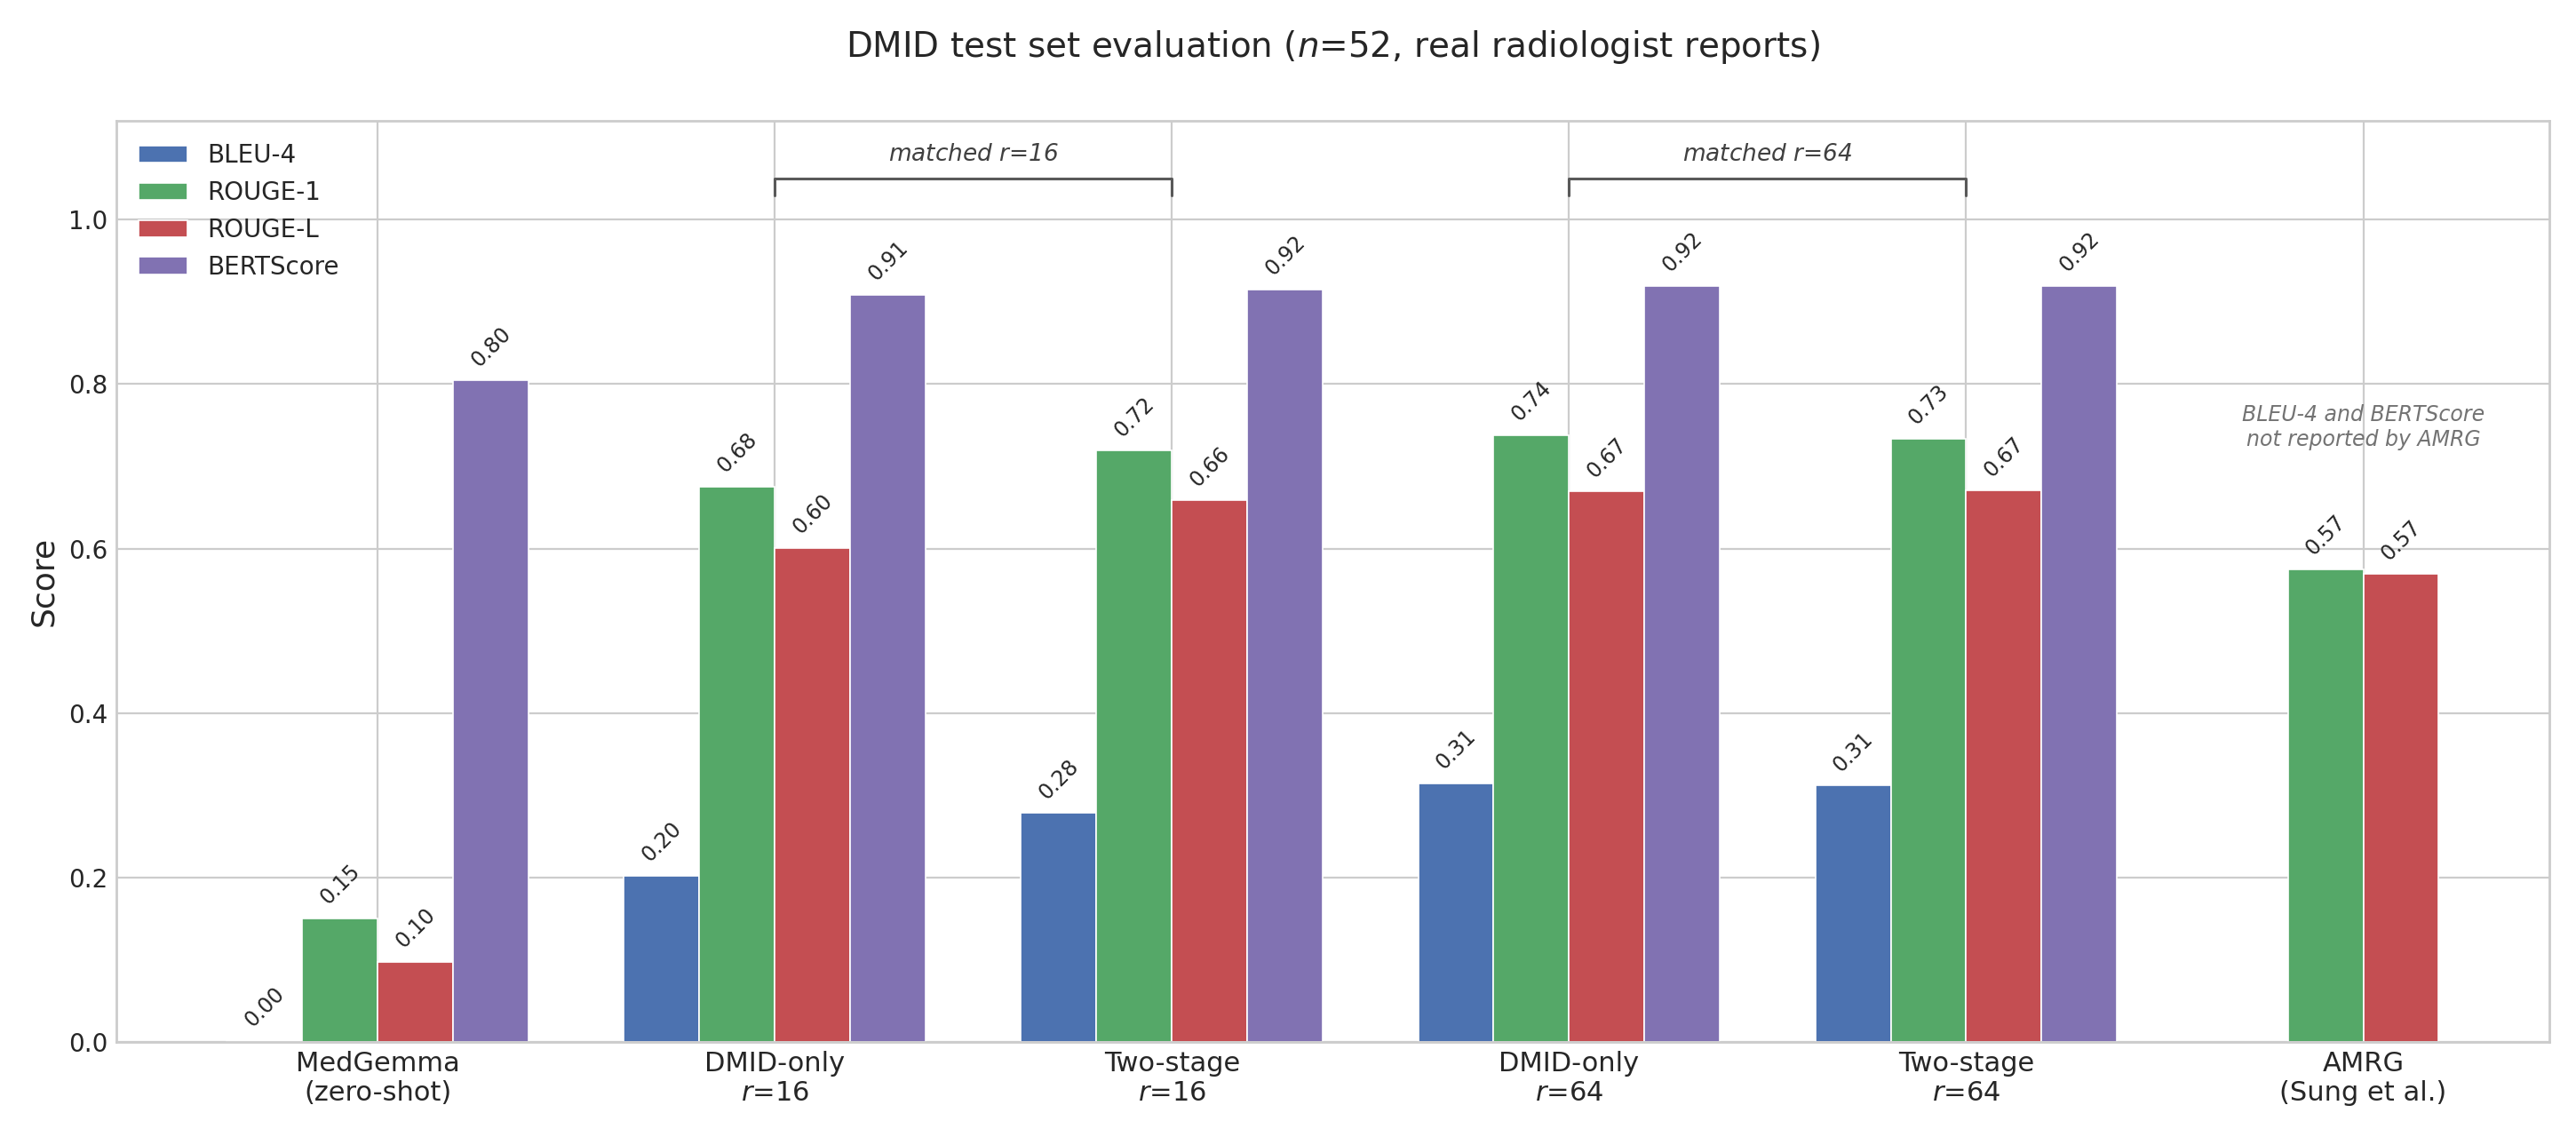
\includegraphics[width=\textwidth]{fig_dmid_ablation.png}
\caption{DMID test set comparison across key methods ($n=52$). Our two-stage approach outperforms all baselines including AMRG across BLEU-4, ROUGE-L, and METEOR.}
\label{fig:dmid_bar}
\end{figure}
\subsection*{Clinical Metric Evaluation}

Table~\ref{tab:clinical} presents clinical quality metrics. In this evaluation, the model must predict clinical attributes directly from mammographic images without any BI-RADS input.

\begin{table}[H]
\centering
\caption{Clinical quality metrics on DMID test set ($n=52$).}
\label{tab:clinical}
\begin{tabular}{lcccc}
\toprule
\textbf{Method} & \textbf{BI-RADS Acc.} & \textbf{Rec. Acc.} & \textbf{Halluc. Rate} & \textbf{Density Acc.} \\
\midrule
MedGemma-4B (ZS)     & 0.038 & 0.538 & 0.731 & ---   \\
DMID-only (LoRA)      & 0.346 & 0.288 & 0.192 & 1/5   \\
Ours (two-stage)      & 0.308 & 0.250 & 0.212 & \textbf{4/5}  \\
\bottomrule
\end{tabular}
\end{table}

Fine-tuning dramatically reduces hallucination rates from 73.1\% to approximately 20\%. The two-stage model more accurately predicts breast density~\cite{gastounioti2022breast} (4/5 correct ACR predictions vs. 1/5 for DMID-only in qualitative analysis), suggesting that synthetic pretraining on VinDr-Mammo density annotations transfers to improved density characterisation. Average generated report length (42.2 words) closely matches real reports (43.1 words), confirming the model learns appropriate report structure.

\subsection*{BI-RADS Distribution and Per-Category Analysis}

The DMID test set exhibits the following BI-RADS distribution: BI-RADS 1 (21.2\%, $n=11$), BI-RADS 2 (13.5\%, $n=7$), BI-RADS 3 (23.1\%, $n=12$), BI-RADS 4 (28.8\%, $n=15$), and BI-RADS 5 (13.5\%, $n=7$). Breast density distribution spans ACR A (5.8\%), ACR B (46.2\%), ACR C (38.5\%), and ACR D (9.6\%).

The predominance of ACR B density in the test set (46.2\%) provides context for the qualitative observation that our two-stage model consistently predicts ACR B: this reflects both the dataset distribution and knowledge transferred from VinDr-Mammo~\cite{nguyen2023vindr}, where ACR B is similarly prevalent. The DMID-only model's tendency to default to ACR C (despite ACR B being more common) suggests insufficient learning of density characteristics from the limited real training data alone, consistent with findings by Lehman et al.~\cite{lehman2019mammographic} on deep learning-based density assessment.

The moderate overall BI-RADS accuracy ($\sim$31\%) masks substantial variation across categories. Normal cases (BI-RADS 1--2) are more reliably identified than suspicious cases (BI-RADS 4--5), consistent with the clinical difficulty of distinguishing subtle malignant features in mammographic images~\cite{sechopoulos2021artificial}. This per-category variation represents an important direction for future work, potentially addressable through class-balanced training or BI-RADS-specific loss weighting.

The hallucination rate reduction from 73.1\% (zero-shot) to $\sim$20\% (fine-tuned) is clinically significant. In the zero-shot setting, MedGemma-4B~\cite{lin2024medgemma} frequently generates verbose, unstructured responses mentioning findings not present in the image---a behaviour that could erode clinical trust. Fine-tuning on domain-specific data teaches the model to generate concise, structured reports that adhere to the BI-RADS format~\cite{birads2013}, even when the clinical content is imperfect. The two-stage model generates reports averaging 42.2 words, closely matching the 43.1-word average of real radiologist reports, compared to 129.2 words for the zero-shot baseline. This length calibration is an underappreciated benefit of domain-specific fine-tuning.

\subsection*{Data Efficiency Analysis}

Figure~\ref{fig:efficiency} and Table~\ref{tab:efficiency} present the data efficiency analysis across varying amounts of real training data.

\begin{table}[H]
\centering
\caption{Data efficiency: performance as a function of real training examples $N$. $\Delta$ denotes relative improvement of two-stage over DMID-only.}
\label{tab:efficiency}
\begin{tabular}{rcccccc}
\toprule
& \multicolumn{2}{c}{\textbf{ROUGE-L}} & \multicolumn{2}{c}{\textbf{ROUGE-1}} & \multicolumn{2}{c}{\textbf{BLEU-4}} \\
\cmidrule(lr){2-3} \cmidrule(lr){4-5} \cmidrule(lr){6-7}
$N$ & DMID-only & Two-stage & DMID-only & Two-stage & DMID-only & Two-stage \\
\midrule
50  & 0.502 & 0.522\;(+4.0\%) & 0.604 & 0.591 & 0.093 & 0.121 \\
100 & 0.542 & 0.570\;(+5.1\%) & 0.618 & 0.644 & 0.103 & 0.135 \\
200 & 0.560 & 0.599\;(+7.0\%) & 0.639 & 0.665 & 0.149 & 0.184 \\
407 & 0.615 & \textbf{0.662}\;(+7.6\%) & 0.686 & \textbf{0.724} & 0.221 & \textbf{0.307} \\
\bottomrule
\end{tabular}
\end{table}

Two key findings emerge. First, synthetic pretraining benefit increases with real data (from +4.0\% to +7.6\%), suggesting complementarity. Second, the two-stage model with 200 real examples (ROUGE-L: 0.599) approaches the DMID-only model with 407 examples (0.615), indicating $\sim$2$\times$ data savings. Notably, two-stage with only 100 examples (0.570) already surpasses the AMRG benchmark~\cite{sung2025} (0.569).


\begin{figure}[H]
\centering
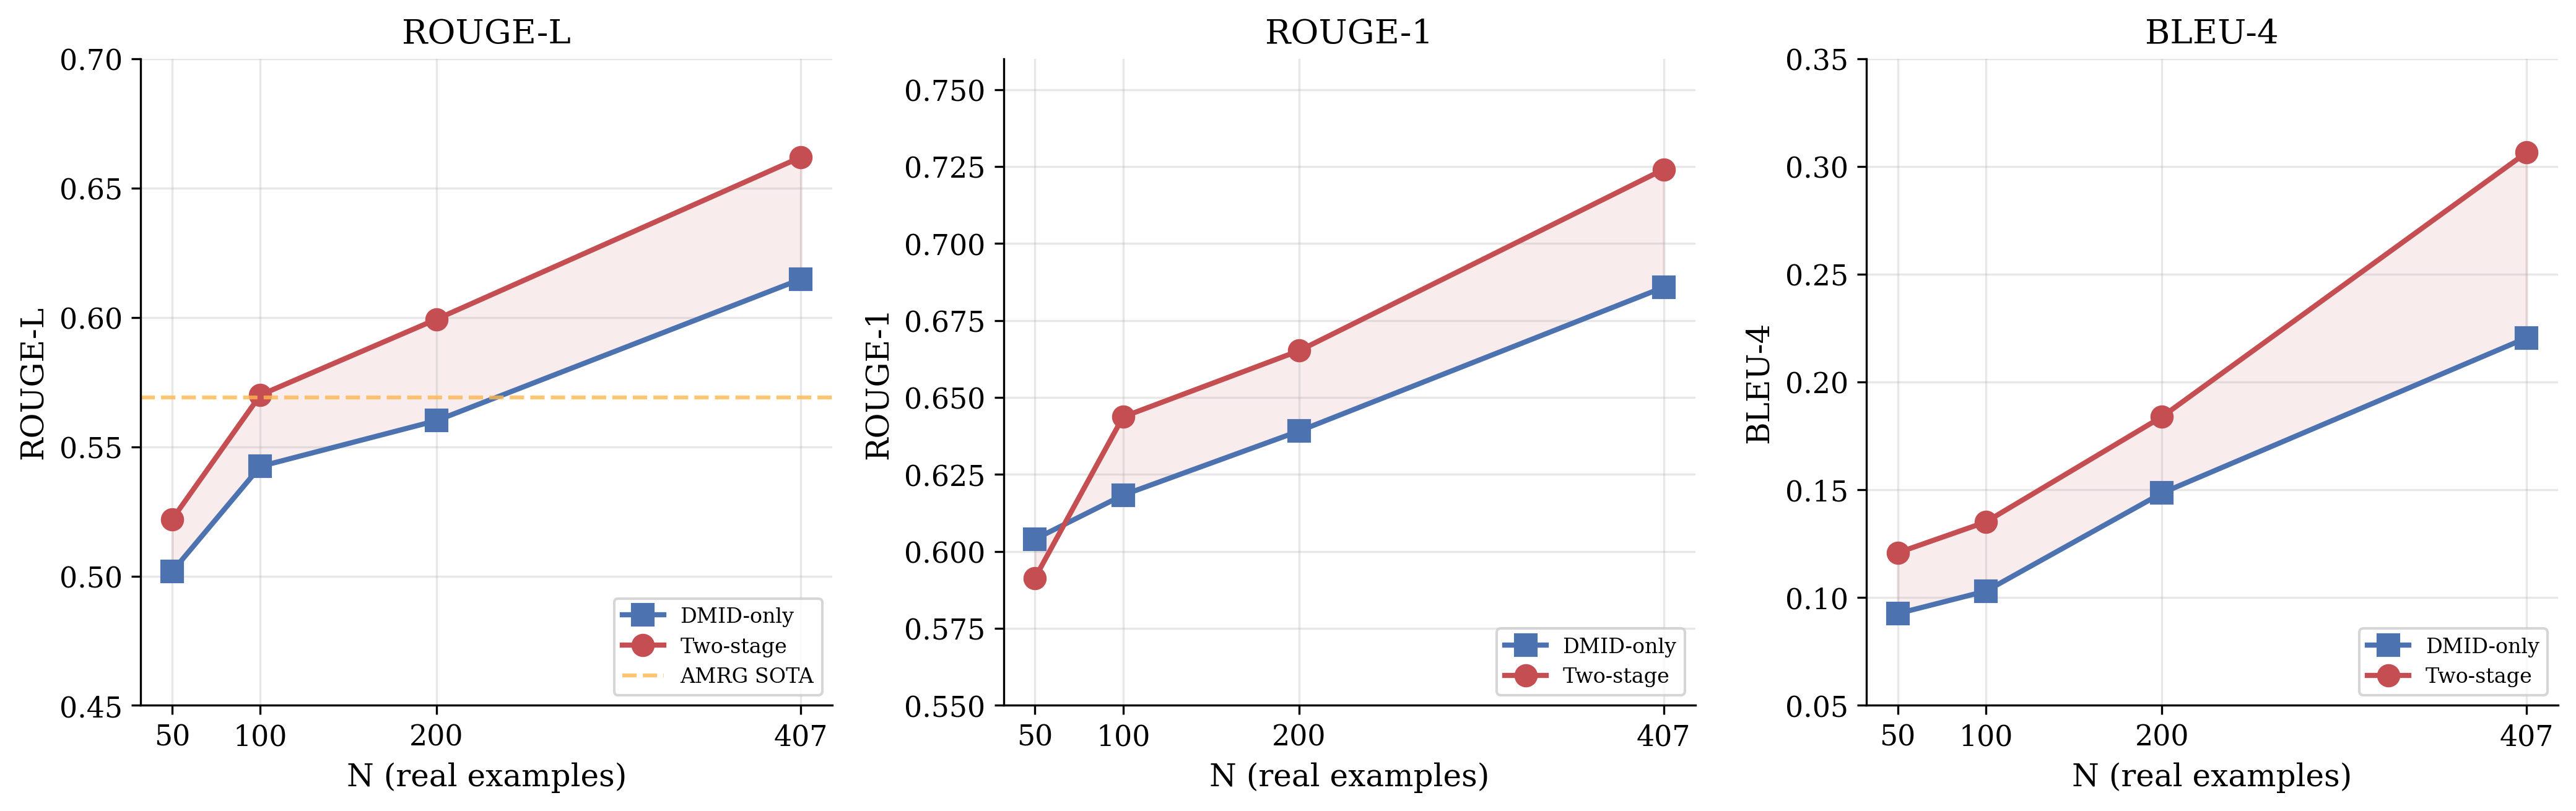
\includegraphics[width=\textwidth]{fig_data_efficiency.png}
\caption{Data efficiency analysis. Synthetic pretraining consistently improves performance and the benefit grows with more real data. Two-stage with $N=100$ surpasses the AMRG SOTA (dashed line).}
\label{fig:efficiency}
\end{figure}

\subsection*{Training Dynamics}

Figure~\ref{fig:curves} compares training dynamics. The two-stage model starts with lower initial training loss (3.33 vs. 4.00) and achieves lower best validation loss (0.655 vs. 0.669), confirming that synthetic pretraining provides a more favourable initialisation, consistent with transfer learning theory~\cite{pan2010transfer}.


\begin{figure}[H]
\centering
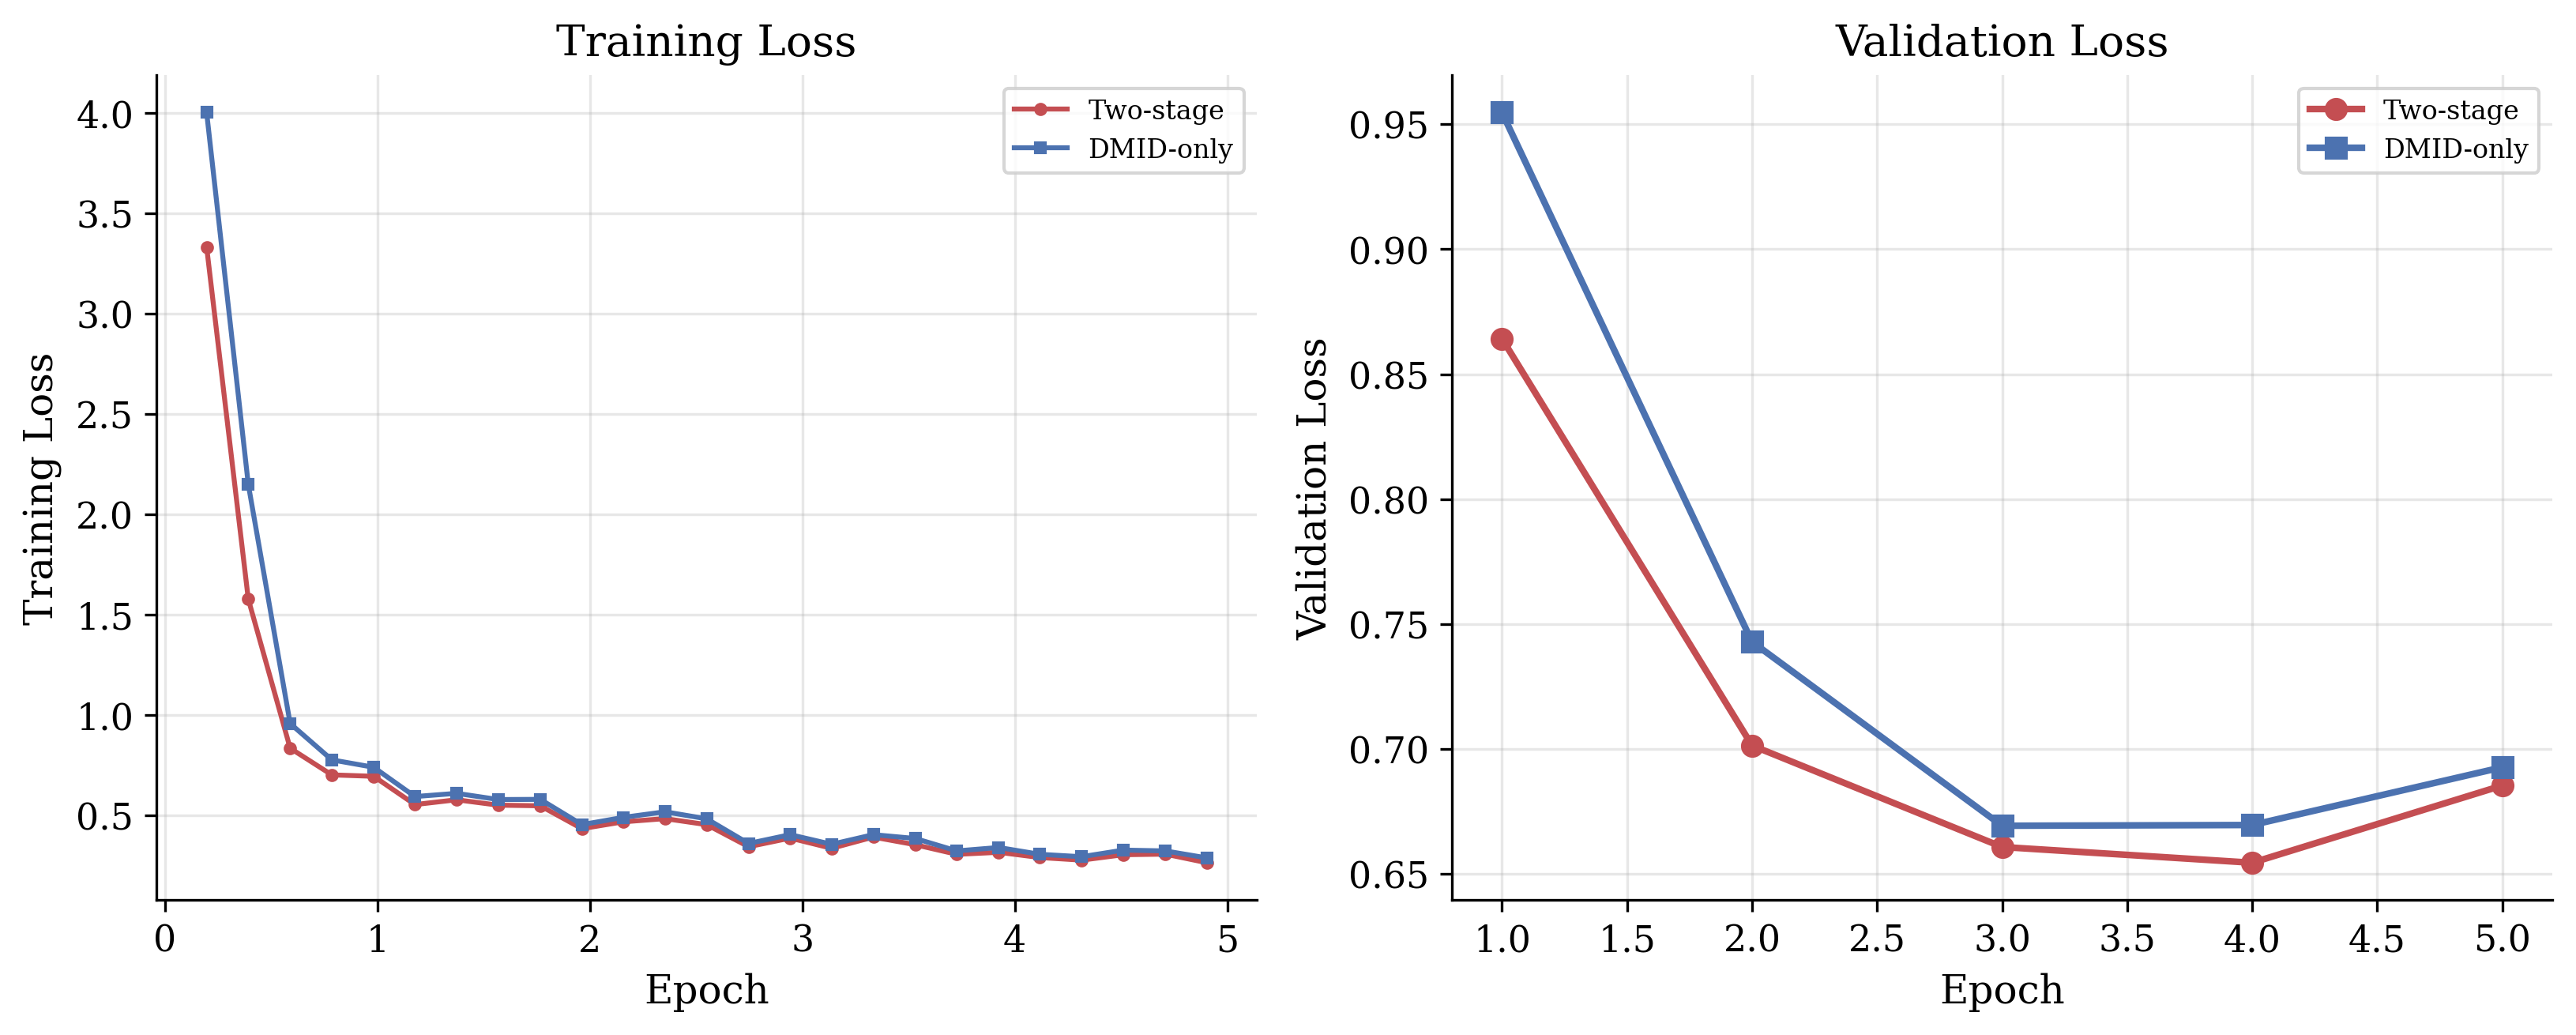
\includegraphics[width=\textwidth]{fig_training_curves.png}
\caption{Training dynamics. Two-stage benefits from lower initial loss and achieves lower best validation loss (0.655 vs. 0.669).}
\label{fig:curves}
\end{figure}

\subsection*{Qualitative Analysis}

Table~\ref{tab:qualitative} presents representative generated reports with colour-coded clinical term evaluation: \textcolor{correct}{correct terms (blue)}, \textcolor{incorrect}{incorrect terms (red)}, and \textcolor{hallucinated}{hallucinated terms (green)}. Each example includes the corresponding mammographic image alongside the ground-truth and generated reports.

\begin{table}[H]
\centering
\caption{Qualitative comparison of generated mammography reports with corresponding mammographic images. Clinical terms: \textcolor{correct}{correct (blue)}, \textcolor{incorrect}{incorrect (red)}, \textcolor{hallucinated}{unseen/hallucinated (green)}.}
\label{tab:qualitative}
\small
\begin{tabularx}{\textwidth}{p{1.8cm}p{1.2cm}X}
\toprule
\textbf{Image} & \textbf{Method} & \textbf{Generated Report} \\
\midrule
\multicolumn{3}{l}{\textbf{Example 1: Img462 --- Normal breast (BI-RADS 1) --- Correct generation}} \\
\midrule
\multirow{4}{*}{\includegraphics[width=1.6cm]{mammo_462.png}}
& \textbf{GT} & BC: \textcolor{correct}{fibro fatty and glandular (ACR B)}. F: \textcolor{correct}{No abnormal soft opacity or microcalcifications}. \textcolor{correct}{Skin and nipple appear normal}. \textcolor{correct}{BIRADS: 1} \\
\addlinespace
& \textbf{Ours} & BC: \textcolor{correct}{fibro fatty and glandular (ACR B)}. F: \textcolor{correct}{No abnormal soft opacity or microcalcification}. \textcolor{correct}{Skin and nipple appear normal}. \textcolor{correct}{BIRADS: 1} \\
\addlinespace
& \textbf{DMID} & BC: \textcolor{incorrect}{fibro glandular (ACR C)}. F: \textcolor{correct}{No abnormal soft opacity or microcalcification}. \textcolor{correct}{Skin and nipple appear normal}. \textcolor{correct}{BIRADS: 1} \\
\addlinespace
& \textbf{ZS} & \textcolor{incorrect}{The right breast appears to have a mix of dense and non-dense tissue}... \textcolor{hallucinated}{[verbose, unstructured, >130 words]} \\
\midrule
\multicolumn{3}{l}{\textbf{Example 2: Img461 --- Normal breast (BI-RADS 1) --- Failure case}} \\
\midrule
\multirow{3}{*}{\includegraphics[width=1.6cm]{mammo_461.png}}
& \textbf{GT} & BC: \textcolor{correct}{fibro fatty and glandular (ACR B)}. F: \textcolor{correct}{No abnormal soft opacity}. \textcolor{correct}{Few small benign looking axillary node}. \textcolor{correct}{BIRADS: 1} \\
\addlinespace
& \textbf{Ours} & BC: \textcolor{correct}{fibro fatty and glandular (ACR B)}. F: \textcolor{hallucinated}{a small well defined soft opacity} suggests \textcolor{incorrect}{probably benign lesion}. \textcolor{incorrect}{BIRADS: 3} \\
\addlinespace
& \textbf{DMID} & BC: \textcolor{incorrect}{fibro glandular (ACR C)}. F: \textcolor{hallucinated}{a large irregular soft opacity with spiculated margin} suggests \textcolor{incorrect}{high suspicious malignant lesion}. \textcolor{incorrect}{BIRADS: 4c} \\
\midrule
\multicolumn{3}{l}{\textbf{Example 3: Img463 --- Normal breast (BI-RADS 1) --- Density comparison}} \\
\midrule
\multirow{3}{*}{\includegraphics[width=1.6cm]{mammo_463.png}}
& \textbf{GT} & BC: \textcolor{correct}{fibro fatty and glandular (ACR C)}. F: \textcolor{correct}{No abnormal soft opacity or microcalcifications}. \textcolor{correct}{No significant axillary adenopathy}. \textcolor{correct}{BIRADS: 1} \\
\addlinespace
& \textbf{Ours} & BC: \textcolor{incorrect}{fibro fatty and glandular (ACR B)}. F: \textcolor{correct}{No abnormal soft opacity or microcalcification}. \textcolor{correct}{No significant axillary adenopathy}. \textcolor{correct}{BIRADS: 1} \\
\addlinespace
& \textbf{DMID} & BC: \textcolor{correct}{fibro glandular (ACR C)}. F: \textcolor{correct}{No abnormal soft opacity or microcalcification}. \textcolor{correct}{No significant axillary adenopathy}. \textcolor{correct}{BIRADS: 1} \\
\bottomrule
\end{tabularx}
\end{table}

Example~1 demonstrates near-perfect generation by our two-stage model, with all clinical terms matching the ground truth. Example~2 illustrates a clinically significant failure mode: while both fine-tuned models hallucinate findings for this normal breast, DMID-only predicts BI-RADS 4c (requiring biopsy) whereas our model predicts BI-RADS 3 (requiring follow-up)---a substantially less clinically harmful error. Example~3 shows that our model consistently predicts ACR B density while DMID-only defaults to ACR C, reflecting the density knowledge transferred from synthetic pretraining on VinDr-Mammo~\cite{nguyen2023vindr}.

\subsection*{LoRA Hyperparameter Ablation}

Table~\ref{tab:lora} presents LoRA~\cite{hu2022lora} rank and scaling factor ablation for Stage~2, with Stage~1 held constant at $r=16, \alpha=32$.

\begin{table}[H]
\centering
\caption{LoRA hyperparameter ablation on DMID test set. Stage~1 uses $r=16, \alpha=32$; Stage~2 varies. Best values in bold.}
\label{tab:lora}
\begin{tabular}{cccccccc}
\toprule
$r$ & $\alpha$ & \textbf{Params} & \textbf{BLEU-4} & \textbf{ROUGE-1} & \textbf{ROUGE-L} & \textbf{METEOR} & \textbf{CIDEr} \\
\midrule
8  & 16  & 16.4M  & 0.268 & 0.700 & 0.631 & 0.633 & 0.527 \\
8  & 32  & 16.4M  & 0.289 & 0.721 & 0.654 & 0.660 & 0.613 \\
16 & 32  & 32.8M  & 0.278 & 0.719 & 0.659 & 0.657 & 0.639 \\
32 & 32  & 65.5M  & 0.290 & 0.714 & 0.648 & 0.656 & 0.646 \\
32 & 64  & 65.5M  & 0.296 & 0.726 & 0.661 & 0.672 & 0.623 \\
\textbf{64} & \textbf{64} & \textbf{131.1M} & \textbf{0.312} & \textbf{0.734} & \textbf{0.671} & \textbf{0.685} & \textbf{0.729} \\
64 & 128 & 131.1M & 0.268 & 0.728 & 0.666 & 0.671 & 0.687 \\
\bottomrule
\end{tabular}
\end{table}
The ablation reveals several insights. First, increasing rank from $r=8$ to $r=64$ consistently improves CIDEr (0.527 $\rightarrow$ 0.729), suggesting that mammography report generation benefits from higher model capacity. Second, the scaling factor $\alpha$ exhibits a non-monotonic relationship: for $r=64$, $\alpha=64$ outperforms $\alpha=128$ across all metrics, indicating that excessive scaling destabilises training. Third, even the smallest configuration ($r=8$, $\alpha=16$, 16.4M parameters) achieves ROUGE-L of 0.631, substantially outperforming all zero-shot baselines and the AMRG benchmark~\cite{sung2025} (0.569), confirming that the two-stage training paradigm---rather than model capacity alone---drives the primary performance gains. The optimal configuration ($r=64$, $\alpha=64$) requires 131.1M trainable parameters (3.0\% of the full model), representing a 4$\times$ increase over the default $r=16$ configuration while yielding +1.8\% ROUGE-L and +14.1\% CIDEr improvements.


%% ─────────────────────────────────────────────────────────────────
\section*{Discussion}
%% ─────────────────────────────────────────────────────────────────

\textbf{Synthetic data as effective pretraining.} The central finding is that LLM-generated synthetic reports serve as effective pretraining data. The two-stage model outperforms DMID-only despite identical real training data ($p=0.045$). We attribute this to: (1) synthetic pretraining teaches mammography report vocabulary and BI-RADS structure~\cite{birads2013}, and (2) this domain-specific initialisation enables more efficient learning, consistent with deep representation learning principles~\cite{bengio2012deep}, evidenced by lower initial training loss (3.33 vs. 4.00).

\textbf{Comprehensive SOTA comparison.} Our approach outperforms all nine evaluated methods spanning four architectural paradigms. Against AMRG~\cite{sung2025} (the previous SOTA), improvements are consistent: ROUGE-L +17.9\%, METEOR +11.4\%, CIDEr +25.3\%. Notably, pipeline approaches (CLIP~\cite{radford2021clip}+GPT2~\cite{radford2019gpt2}) achieve competitive ROUGE-L (0.613) but lower CIDEr, suggesting that end-to-end VLM fine-tuning produces more clinically coherent reports.

\textbf{Data efficiency.} Synthetic pretraining reduces real data requirements by $\sim$2$\times$. With only 100 real examples, our approach matches the AMRG benchmark---critical for clinical settings where paired data is scarce. The benefit grows with data size (+4\% at $N=50$ to +7.6\% at $N=407$), indicating synthetic and real data are complementary. This finding complements recent work on transfer learning for medical imaging~\cite{zhuang2021survey}.

\textbf{Clinical quality.} Fine-tuning reduces hallucination from 73.1\% to $\sim$20\%. Qualitative analysis reveals that even in failure cases, the two-stage model produces less clinically harmful errors (BI-RADS 3 vs. 4c for a BI-RADS 1 case). The model consistently predicts density more accurately (ACR B matching ground truth) than DMID-only (defaulting to ACR C), suggesting knowledge transfer from VinDr-Mammo~\cite{nguyen2023vindr} density annotations, consistent with findings on deep learning-based density assessment~\cite{lehman2019mammographic, gastounioti2022breast}. The attention mechanisms explored in our prior work~\cite{esen2025multitask} and Grad-CAM~\cite{selvaraju2017gradcam} interpretability~\cite{esen2025rl} provide complementary approaches to building clinician trust in AI-generated reports.

\textbf{Architectural paradigm comparison.} Our evaluation spans four distinct architectural paradigms. Zero-shot VLMs (LLaVA~\cite{liu2024llava}, Qwen~\cite{wang2024qwen2vl}, MedGemma~\cite{lin2024medgemma}) uniformly perform poorly on mammography, with ROUGE-L below 0.15, indicating that general-purpose VLM pretraining does not transfer to specialised mammographic reporting. Pipeline approaches (CLIP+GPT2) achieve surprisingly competitive results after fine-tuning (ROUGE-L: 0.571--0.613). However, end-to-end VLM fine-tuning with our two-stage approach consistently outperforms pipeline methods across all metrics, particularly CIDEr (0.729), indicating superior clinical coherence.

\textbf{Comparison with AMRG methodology.} While both our approach and AMRG~\cite{sung2025} fine-tune MedGemma-4B~\cite{lin2024medgemma} with LoRA~\cite{hu2022lora} on the DMID dataset, several methodological differences contribute to our superior performance. First, our two-stage pretraining provides domain-adapted initialisation absent from AMRG's direct fine-tuning. Second, our LoRA ablation identifies $r=64$, $\alpha=64$ as optimal, compared to AMRG's $r=32$, $\alpha=16$---a configuration we find suboptimal. Third, AMRG does not incorporate synthetic data augmentation or RAG~\cite{lewis2020rag}, both of which contribute to our framework's robustness.

\textbf{LoRA configuration analysis.} Our systematic ablation across seven LoRA~\cite{hu2022lora} configurations reveals that the optimal rank ($r=64$, $\alpha=64$) substantially outperforms the commonly used default ($r=16$, $\alpha=32$), particularly on CIDEr (+14.1\%). We attribute this to the two-stage training paradigm: because Stage~1 pretraining already provides a strong initialisation, Stage~2 benefits from higher-capacity LoRA adapters that can capture fine-grained stylistic differences between synthetic and real reports.

\textbf{Context within broader research.} Our results complement recent clinical AI deployment studies~\cite{dembrower2020effect, salim2020external, aboutalib2018deep}, suggesting that automated report generation could reduce radiologist workload while maintaining diagnostic quality. The detection capabilities demonstrated by Shen et al.~\cite{shen2019deep} and Ribli et al.~\cite{ribli2018detecting} in Scientific Reports, along with the feature extraction approaches by Aitimov et al.~\cite{aitimov2025feature} from Kazakhstan, highlight the growing maturity of deep learning for mammography analysis. Modern architectures including ResNet~\cite{he2016deep}, DenseNet~\cite{huang2017densely}, transformers~\cite{vaswani2017attention}, and Vision Transformers~\cite{dosovitskiy2021vit} have been foundational to this progress. Unlike chest X-ray report generation which benefits from large-scale datasets~\cite{johnson2019mimiccxr}, mammography faces severe data scarcity, making our synthetic-to-real approach particularly valuable.

\textbf{RAG trade-offs.} In Stage~1, RAG decreased NLP metrics while maintaining clinical quality, reflecting n-gram-based evaluation limitations for clinical text. Future work should incorporate RadGraph F1 for entity-level clinical evaluation.

\textbf{Limitations.} The DMID test set is small ($n=52$); larger paired datasets would strengthen conclusions. Formal radiologist evaluation is essential before clinical deployment. Single-view processing limits multi-view reasoning. The moderate BI-RADS accuracy ($\sim$31\%) reflects the difficulty of predicting BI-RADS from images alone. We additionally evaluated mammography-specific image preprocessing (Otsu thresholding, ROI cropping, laterality matching, CLAHE) but observed no improvement in ROUGE-L (0.662 vs. 0.671) and reduced CIDEr (0.551 vs. 0.729), suggesting that SigLIP's~\cite{zoph2020siglip} vision encoder handles raw mammographic inputs robustly without domain-specific preprocessing.

\textbf{Future work.} Multi-view integration; BI-RADS-guided constrained decoding; extension to other low-resource medical imaging domains; formal radiologist evaluation; reinforcement learning from human feedback (RLHF) building on our prior RL work~\cite{esen2025rl}.

\section*{Conclusion}

We present a two-stage synthetic-to-real transfer learning framework for automated mammography report generation that addresses the fundamental data scarcity problem limiting VLM development in this domain. Our approach introduces three key innovations: (1) a label-to-report synthesis pipeline using Llama-3.1-8B~\cite{dubey2024llama3} that generates clinically validated training data from structured BI-RADS~\cite{birads2013} annotations, (2) a two-stage training paradigm~\cite{pan2010transfer} where synthetic pretraining provides domain-specific initialisation for subsequent real-data fine-tuning, and (3) a BI-RADS-grounded RAG module~\cite{lewis2020rag} for clinical knowledge integration.

By pretraining MedGemma-4B~\cite{lin2024medgemma} with multimodal LoRA~\cite{hu2022lora} on 400 synthetic reports and fine-tuning on 407 real DMID~\cite{oza2024} reports with optimised LoRA configuration ($r=64$, $\alpha=64$), our approach achieves ROUGE-L~\cite{lin2004rouge} of 0.671, METEOR~\cite{banerjee2005meteor} of 0.685, CIDEr~\cite{vedantam2015cider} of 0.729, and BERTScore~\cite{zhang2020bertscore} of 0.917 on the DMID benchmark. These results surpass the previously reported AMRG~\cite{sung2025} state-of-the-art across all metrics, with improvements of +17.9\% in ROUGE-L, +11.4\% in METEOR, and +25.3\% in CIDEr.

Our data efficiency analysis reveals that synthetic pretraining reduces real data requirements by approximately 2$\times$: the two-stage model trained on just 100 real examples already surpasses the AMRG benchmark. Clinical analysis shows that fine-tuning reduces hallucination rates from 73.1\% to approximately 21\%, while qualitative evaluation reveals that even in failure cases, the two-stage model produces less clinically harmful errors than models trained on real data alone. The systematic LoRA ablation across seven configurations provides practical guidance for hyperparameter selection in medical VLM fine-tuning. Our framework provides a practical, reproducible, and scalable foundation for mammography report generation, and the demonstrated synthetic-to-real transfer learning paradigm may serve as a general strategy for low-resource medical AI development. All code, synthetic datasets, and trained model weights are publicly released to facilitate future research and clinical translation.

%% ─────────────────────────────────────────────────────────────────
\section*{Data Availability}
%% ─────────────────────────────────────────────────────────────────

VinDr-Mammo~\cite{nguyen2023vindr} and CBIS-DDSM~\cite{lee2017curated} are available on Kaggle. DMID~\cite{oza2024} is available on Figshare and Kaggle. Synthetic datasets and model weights will be released upon acceptance.

\section*{Code Availability}

All code is available at \url{https://github.com/ganiesenov/two-stage-mammo-vlm}.

\section*{Author Contributions}

G.E. conceived the study, designed the methodology, implemented the full experimental pipeline, performed data preprocessing, model training, and evaluation, conducted quantitative and qualitative analyzes, and wrote the original manuscript draft.
 
M.N. supervised the research, contributed to the conceptual development of the study, provided guidance on methodology and experimental design, validated the results, and critically reviewed and edited the manuscript.
 
J.A. contributed to the clinical interpretation of results, assisted in data collection and validation, and provided domain-specific expertise in mammography and radiology.
 
L.L.P. contributed to methodological refinement, supported analysis and interpretation of results, and participated in manuscript review and editing.
 
All authors discussed the results, contributed to the final manuscript, and approved the submitted version.

\section*{Competing Interests}

The authors declare no competing interests.

\section*{Acknowledgements}

The authors thank the creators of VinDr-Mammo, CBIS-DDSM, and DMID for making their datasets publicly available, and Google for providing access to MedGemma-4B.

\section*{Funding}

This work was funded by the Committee of Science of the Ministry of Science and Higher Education of the Republic of Kazakhstan under Grant No.\ AP22788239.

\bibliography{references}

\end{document}